\documentclass[paper=letter,11pt]{scrartcl}

\KOMAoptions{headinclude=true, footinclude=false}
\KOMAoptions{DIV=14, BCOR=5mm}
\KOMAoptions{numbers=noendperiod}
\KOMAoptions{parskip=half}
\addtokomafont{disposition}{\rmfamily}
\addtokomafont{part}{\LARGE}
\addtokomafont{descriptionlabel}{\rmfamily}
%\setkomafont{pageheadfoot}{\normalsize\sffamily}
\setkomafont{pagehead}{\normalsize\rmfamily}
%\setkomafont{publishers}{\normalsize\rmfamily}
\setkomafont{caption}{\normalfont\small}
\setcapindent{0pt}
\deffootnote[1em]{1em}{1em}{\textsuperscript{\thefootnotemark}\ }


\usepackage{amsmath}
\usepackage[varg]{txfonts}
\usepackage[T1]{fontenc}
\usepackage{graphicx}
\usepackage{xcolor}
\usepackage[american]{babel}
% hyperref is needed in many places, so include it here
\usepackage{hyperref}

\usepackage{xspace}
\usepackage{multirow}
\usepackage{float}


\usepackage{braket}
\usepackage{bbm}
\usepackage{relsize}
\usepackage{tcolorbox}

\def\ketY{\ensuremath{\ket {\Psi}}}
\def\iGeV{\ensuremath{\textrm{GeV}^{-1}}}
%\def\mp{\ensuremath{m_{\textrm{proton}}}}
\def\rp{\ensuremath{r_{\textrm{proton}}}}
\def\me{\ensuremath{m_{\textrm{electron}}}}
\def\aG{\ensuremath{\alpha_G}}
\def\rAtom{\ensuremath{r_{\textrm{atom}}}}
\def\rNucl{\ensuremath{r_{\textrm{nucleus}}}}
\def\GN{\ensuremath{\textrm{G}_\textrm{N}}}
\def\ketX{\ensuremath{\ket{\vec{x}}}}
\def\ve{\ensuremath{\vec{\epsilon}}}


\def\ABCDMatrix{\ensuremath{\begin{pmatrix} A &  B  \\ C  & D \end{pmatrix}}}
\def\xyprime{\ensuremath{\begin{pmatrix} x' \\ y' \end{pmatrix}}}
\def\xyprimeT{\ensuremath{\begin{pmatrix} x' &  y' \end{pmatrix}}}
\def\xy{\ensuremath{\begin{pmatrix} x \\ y \end{pmatrix}}}
\def\xyT{\ensuremath{\begin{pmatrix} x & y \end{pmatrix}}}

\def\IMatrix{\ensuremath{\begin{pmatrix} 0 &  1  \\ -1  & 0 \end{pmatrix}}}
\def\IBoostMatrix{\ensuremath{\begin{pmatrix} 0 &  1  \\ 1  & 0 \end{pmatrix}}}
\def\JThree{\ensuremath{\begin{pmatrix}    0 & -i & 0  \\ i & 0  & 0 \\ 0 & 0 & 0 \end{pmatrix}}} 
\def\JTwo{\ensuremath{\begin{bmatrix}    0 & 0 & -i  \\ 0 & 0  & 0 \\ i & 0 & 0 \end{bmatrix}}}
\def\JOne{\ensuremath{\begin{bmatrix}    0 & 0 & 0  \\ 0 & 0  & -i \\ 0 & i & 0 \end{bmatrix}}}
\def\etamn{\ensuremath{\eta_{\mu\nu}}}
\def\Lmn{\ensuremath{\Lambda^\mu_\nu}}
\def\dmn{\ensuremath{\delta^\mu_\nu}}
\def\wmn{\ensuremath{\omega^\mu_\nu}}
\def\be{\begin{equation*}}
\def\ee{\end{equation*}}
\def\bea{\begin{eqnarray*}}
\def\eea{\end{eqnarray*}}
\def\bi{\begin{itemize}}
\def\ei{\end{itemize}}
\def\fmn{\ensuremath{F_{\mu\nu}}}
\def\fMN{\ensuremath{F^{\mu\nu}}}
\def\bc{\begin{center}}
\def\ec{\end{center}}
\def\nus{$\nu$s}

\def\adagger{\ensuremath{a_{p\sigma}^\dagger}}
\def\lineacross{\noindent\rule{\textwidth}{1pt}}

\newcommand{\multiline}[1] {
\begin{tabular} {|l}
#1
\end{tabular}
}

\newcommand{\multilineNoLine}[1] {
\begin{tabular} {l}
#1
\end{tabular}
}



\newcommand{\lineTwo}[2] {
\begin{tabular} {|l}
#1 \\
#2
\end{tabular}
}

\newcommand{\rmt}[1] {
\textrm{#1}
}


%
% Units
%
\def\m{\ensuremath{\rmt{m}}}
\def\GeV{\ensuremath{\rmt{GeV}}}
\def\pt{\ensuremath{p_\rmt{T}}}


\def\parity{\ensuremath{\mathcal{P}}}

\usepackage{cancel}
\usepackage{ mathrsfs }
\def\bigL{\ensuremath{\mathscr{L}}}

\usepackage{ dsfont }



\usepackage{fancyhdr}
\fancyhf{}


\lhead{\Large 33-444} % \hfill Introduction to Particle Physics \hfill Spring 2022}
\chead{\Large Introduction to Particle Physics} % \hfill Spring 2022}
\rhead{\Large Spring 2022} % \hfill Introduction to Particle Physics \hfill Spring 2022}

\begin{document}
\thispagestyle{fancy}

\begin{center}
{\huge \textbf{Lecture 30}}
\end{center}

{\fontsize{14}{16}\selectfont


\textbf{\underline{Recap: $SU(2)_L \times U(1)$}}


Start with:  
\be
\underbrace{\phi_1, \hspace*{0.2in} \phi_2, \hspace*{0.2in} \phi_3, \hspace*{0.2in} \phi_4}_{\rmt{DoF: $4\times 1$ (scalars) }}, \hspace*{0.2in} \underbrace{W^1, \hspace*{0.2in} W^2, \hspace*{0.2in}W^3, \hspace*{0.2in} B}_{\rmt{$4\times 2$ (mass-less spin-1)}}
\ee
So 12 total degrees of freedom.

When $\mu^2 < 0$, left with


\be
\underbrace{h}_{\rmt{DoF: 1}} \hspace*{0.3in} \underbrace{W^+ \hspace*{0.3in} W^- \hspace*{0.3in} Z}_{\rmt{$3 \times 3$ (massive spin 1) }} \hspace*{0.3in} \underbrace{\gamma}_{2}
\ee

Total degrees of freedom 12, as needed!


\be
A_\mu = \frac{1}{\sqrt{g_W^2 + g'^2}}(g'W_\mu^3 + g_W B_\mu)  \equiv \cos \theta_W B_\mu + \sin \theta_W W_\mu^3
\ee

\be
Z_\mu = \frac{1}{\sqrt{g_W^2 + g'^2}}(g_W W_\mu^3 - g' B_\mu)  \equiv -\sin \theta_W B_\mu + \cos \theta_W W_\mu^3
\ee

\be
\frac{g'}{g} = \tan \theta_W  \hspace*{1in} m_\gamma = 0 \hspace*{1in} m_Z = \frac{1}{2} \frac{g}{\cos \theta_W} v
\ee


\be
v^2 = \frac{-\mu^2}{\lambda} \simeq 250 \GeV  \hspace*{1in} \frac{m_W}{m_Z} = \cos \theta_W \hspace*{1in} m_H^2 = 2 \lambda v^2
\ee

Predictions coming from Electro-weak unification.
eg: relationship between W and Z boson masses.


Higgs mechanism on $SU(2)_L \times U(1)$ generates the correct Electro-weak spectra. 

\clearpage

\underline{Comments}
\bi
\item[-] Weak force carriers charged, implies relationship between weak and EM force.
\item[-] Coupling constants not so different $\frac{1}{137}$ vs $\frac{1}{50}$
\item[-] Also strong theoretical arguments that they must be related...Talk about this now
\ei

Can produce pairs of $W$'s from $e^+e^-$ collisions

\be
\underbrace{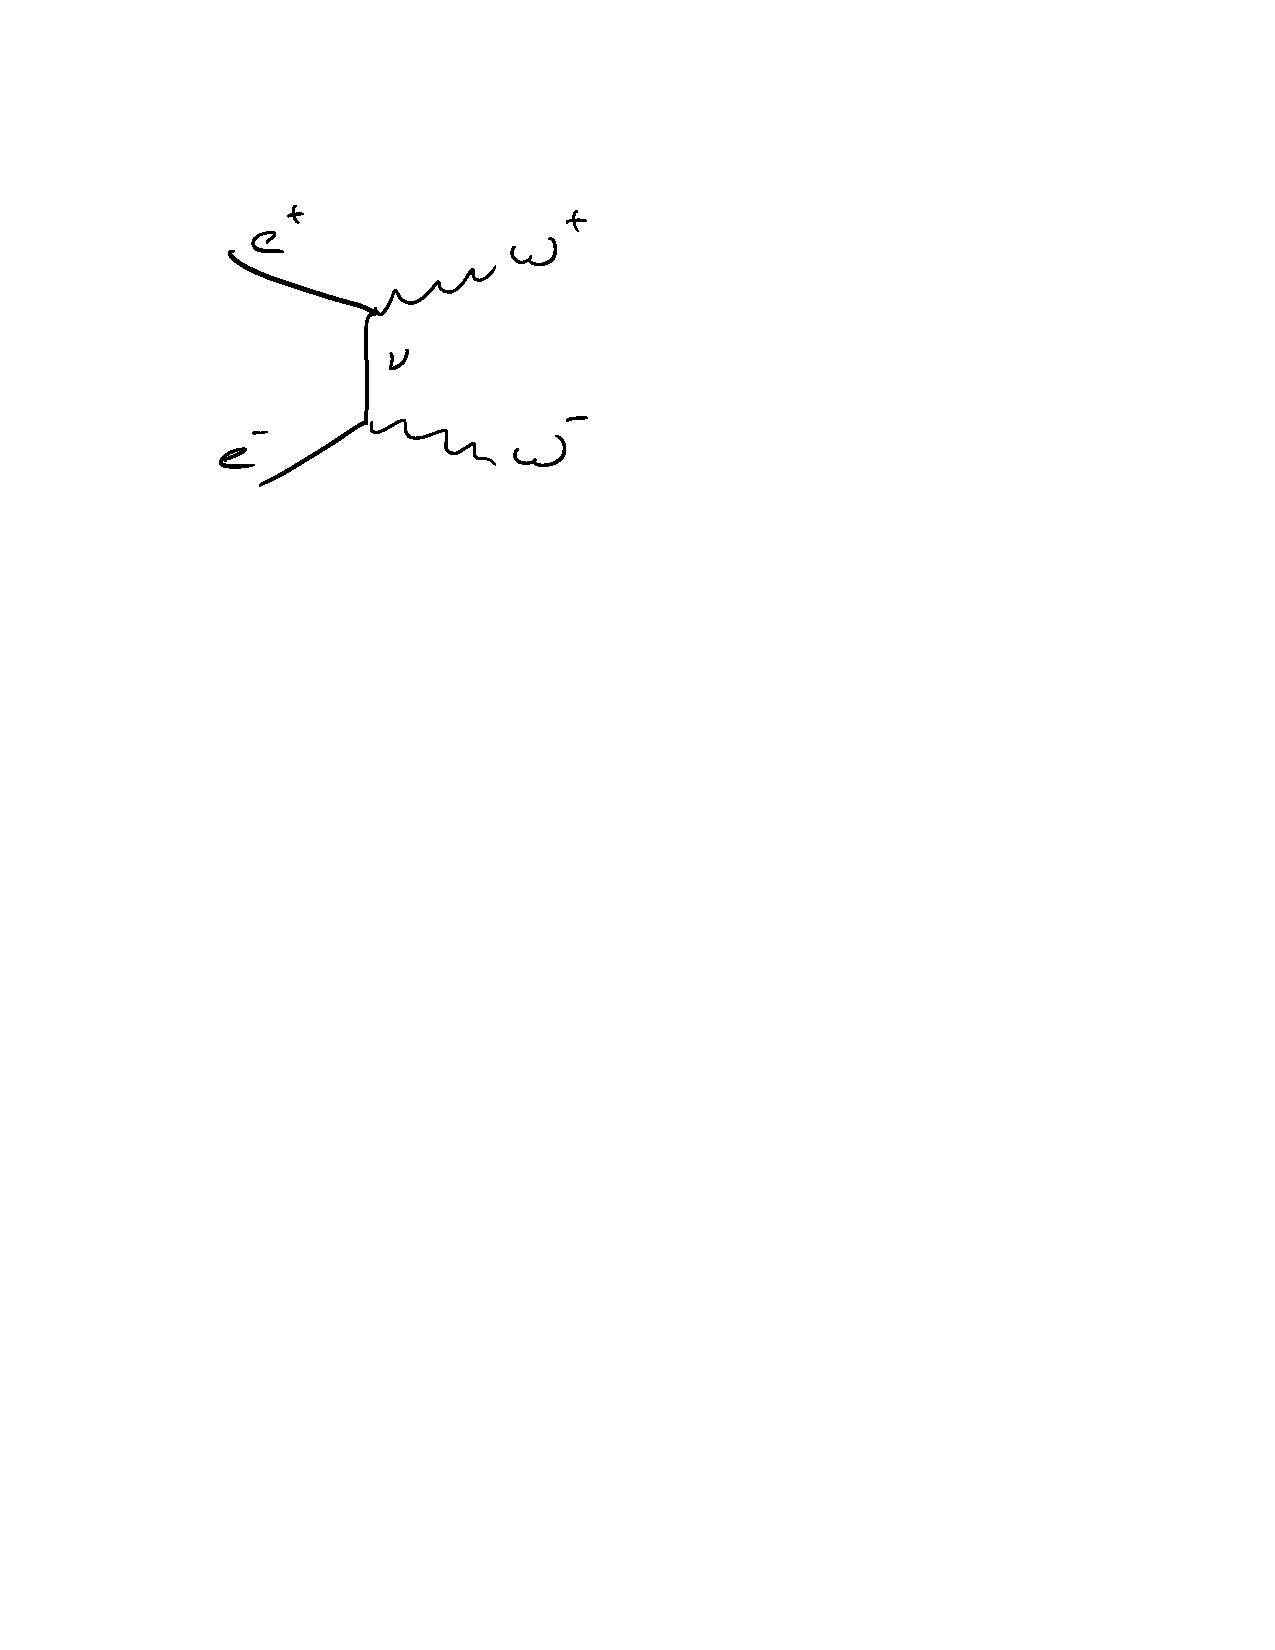
\includegraphics[width=0.3\textwidth]{./eeNuWW.pdf}}_{\rmt{\huge $\sim \alpha_W^2$}}
\hspace*{0.7in}
\underbrace{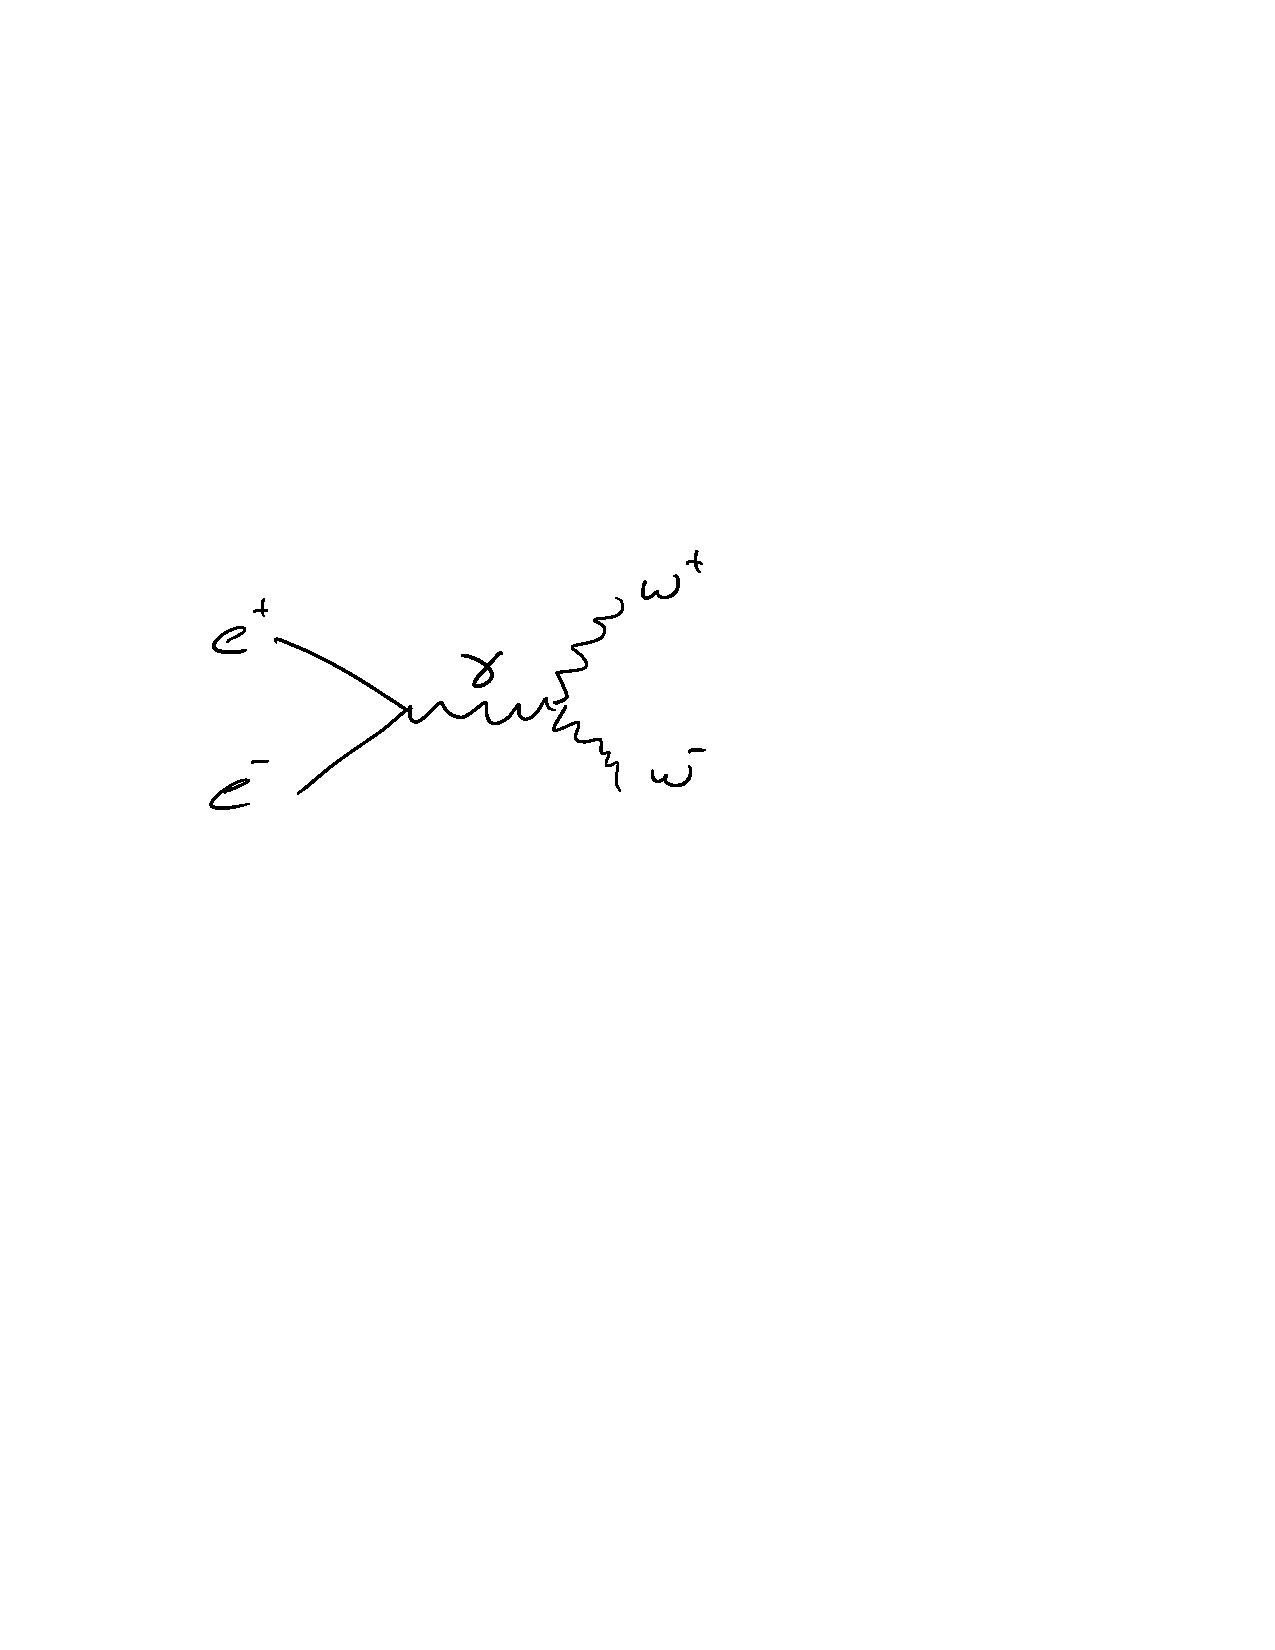
\includegraphics[width=0.4\textwidth]{./eeGammaWW.pdf}}_{\rmt{\huge $\sim \alpha \times \alpha_W$}}
\ee
with these $\sigma$ increases with Energy without limit.
Eventually probability not conserved.  (Calculated WW flux exceeds $e^+e^-$ flux)

Including 3rd diagram resolves problem with negative interference:
\be
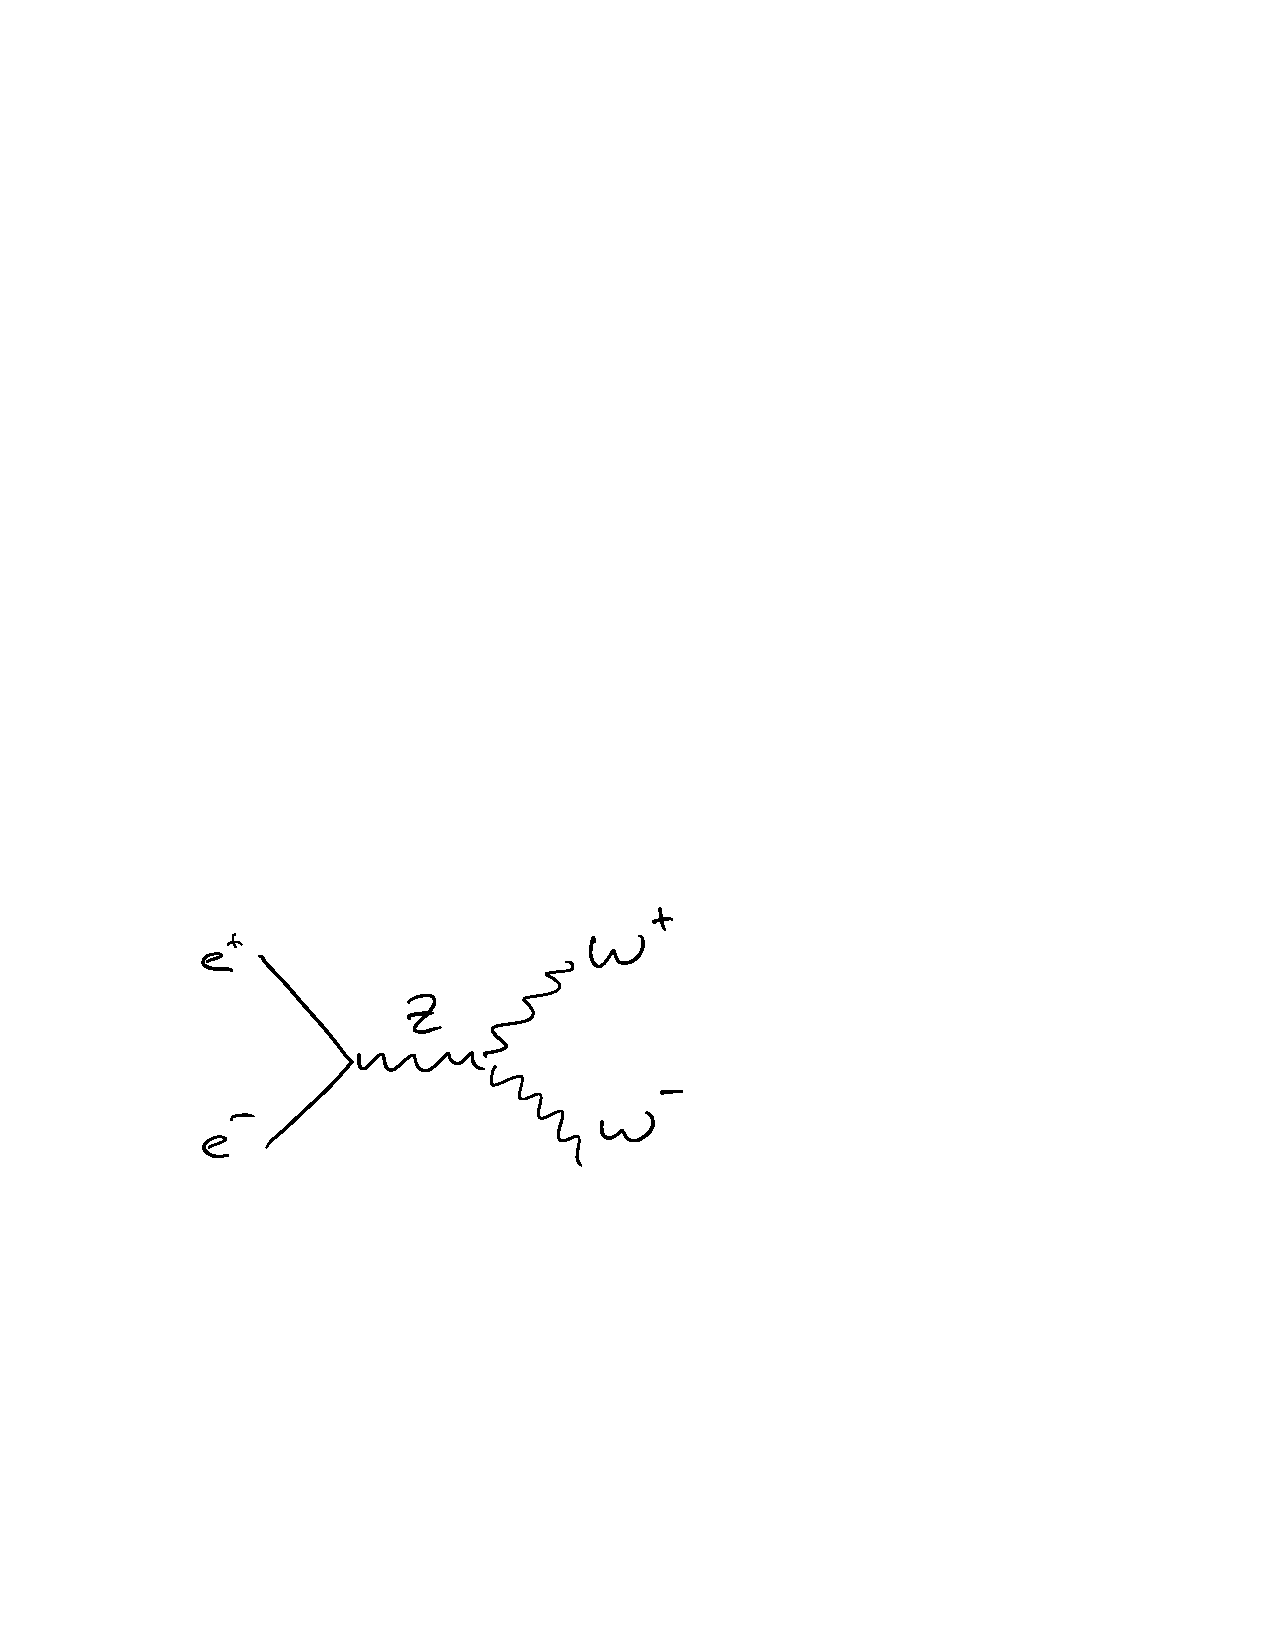
\includegraphics[width=0.4\textwidth]{./eeZWW.pdf}
\ee
Only works because relative couplings are related in very specific way.

\clearpage

\underline{\textbf{Fermion Masses}}

Remarkably, the stupidest Higgs mechanism can also be used to generate Fermion masses... Lets see how. 

Note that a Fermion mass term in the Lagrangian:
\be
-m \psi \psi = -m (\psi_R \psi_L + \psi_L \psi_R )
\ee
does not respect $SU(2)_L$.

$\Rightarrow$ ``bare'' mass terms cannot be included in $\mathcal{L}_{SM}$.

\be
\psi_L = \begin{pmatrix} \nu \\ e \end{pmatrix}_L  \hspace*{1in}  \psi_R = e_R  \hspace*{1in}  \rmt{etc...}
\ee

Now $\phi_\rmt{Higgs}$ is a doublet that transforms under $SU(2)_L$.

So the term $\psi_L \phi_{\rmt{Higgs}}$ is invariant under $SU(2)_L$ (and U(1)).\\
$\Rightarrow$ the term $\psi_L \phi_{\rmt{Higgs}} \psi_R$ is invariant under $SU(2)_L \times U(1)$.


So we are free to add terms like:

\be
\mathcal{L} \supset -g_F \left( \bar{\psi}_L \phi_{\rmt{Higgs}} \psi_R + \bar{\psi}_R \phi^\dagger_{\rmt{Higgs}} \psi_L \right)
\ee
eg:
\be
\mathcal{L} \supset -g_e \left( \begin{pmatrix} \nu_e & e \end{pmatrix}_L   \begin{pmatrix} \phi^+ \\ \phi^0 \end{pmatrix} e_R + e_R \begin{pmatrix} \phi^+ & {\phi^0}^* \end{pmatrix}  \begin{pmatrix} \nu_e \\ e \end{pmatrix}_L \right)
\ee
$g_e$ - refereed to as the ``electron Yukawa'' coupling.  (Coupling constant. not a dimensional mass parameter)\\
Note dimensions on these terms $\Rightarrow$  $g_e$ -dimensionless.

Now, after Electro-weak Symmetry Breaking, $\phi_H \rightarrow \phi = \frac{1}{\sqrt{2}} \begin{pmatrix} 0 \\ v + h(x) \end{pmatrix}$

\be
\mathcal{L} \rightarrow \mathcal{L'} \supset \underbrace{\frac{-g_e}{\sqrt{2}} v \left( e_L e_R + e_R e_L \right)}_{\rmt{Exactly whats needed for mass term!}} -  \frac{g_e}{\sqrt{2}} h(x) \left( e_L e_R + e_R e_L \right) 
\ee

require $g_e = \sqrt{2} \frac{m_e}{v}$ 

Note, not predicted by the Higgs Mechanism, but allowed in gauge invariant way.

\be
\mathcal{L}_e = \underbrace{-m_e e_L e_R}_{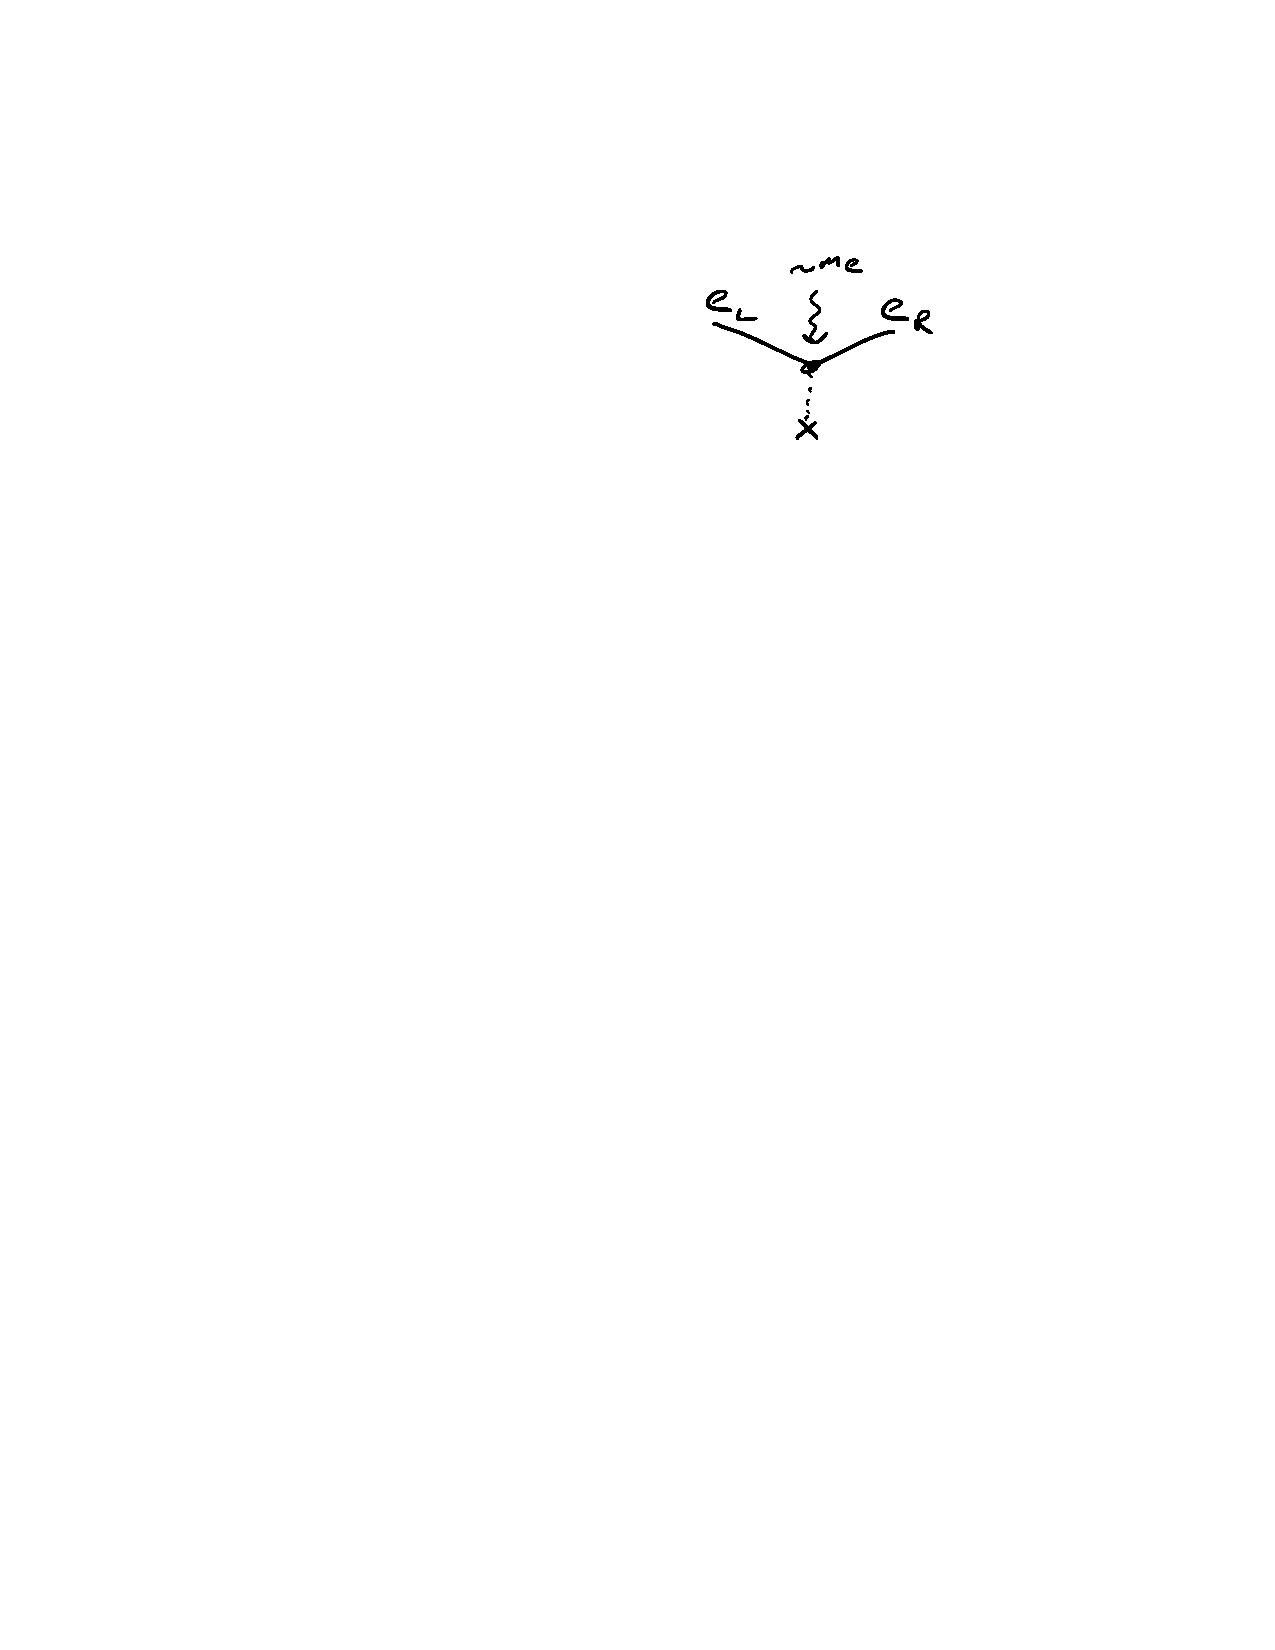
\includegraphics[width=0.2\textwidth]{./electronMass.pdf}} - \underbrace{\frac{m_e}{v} e_R e_L h}_{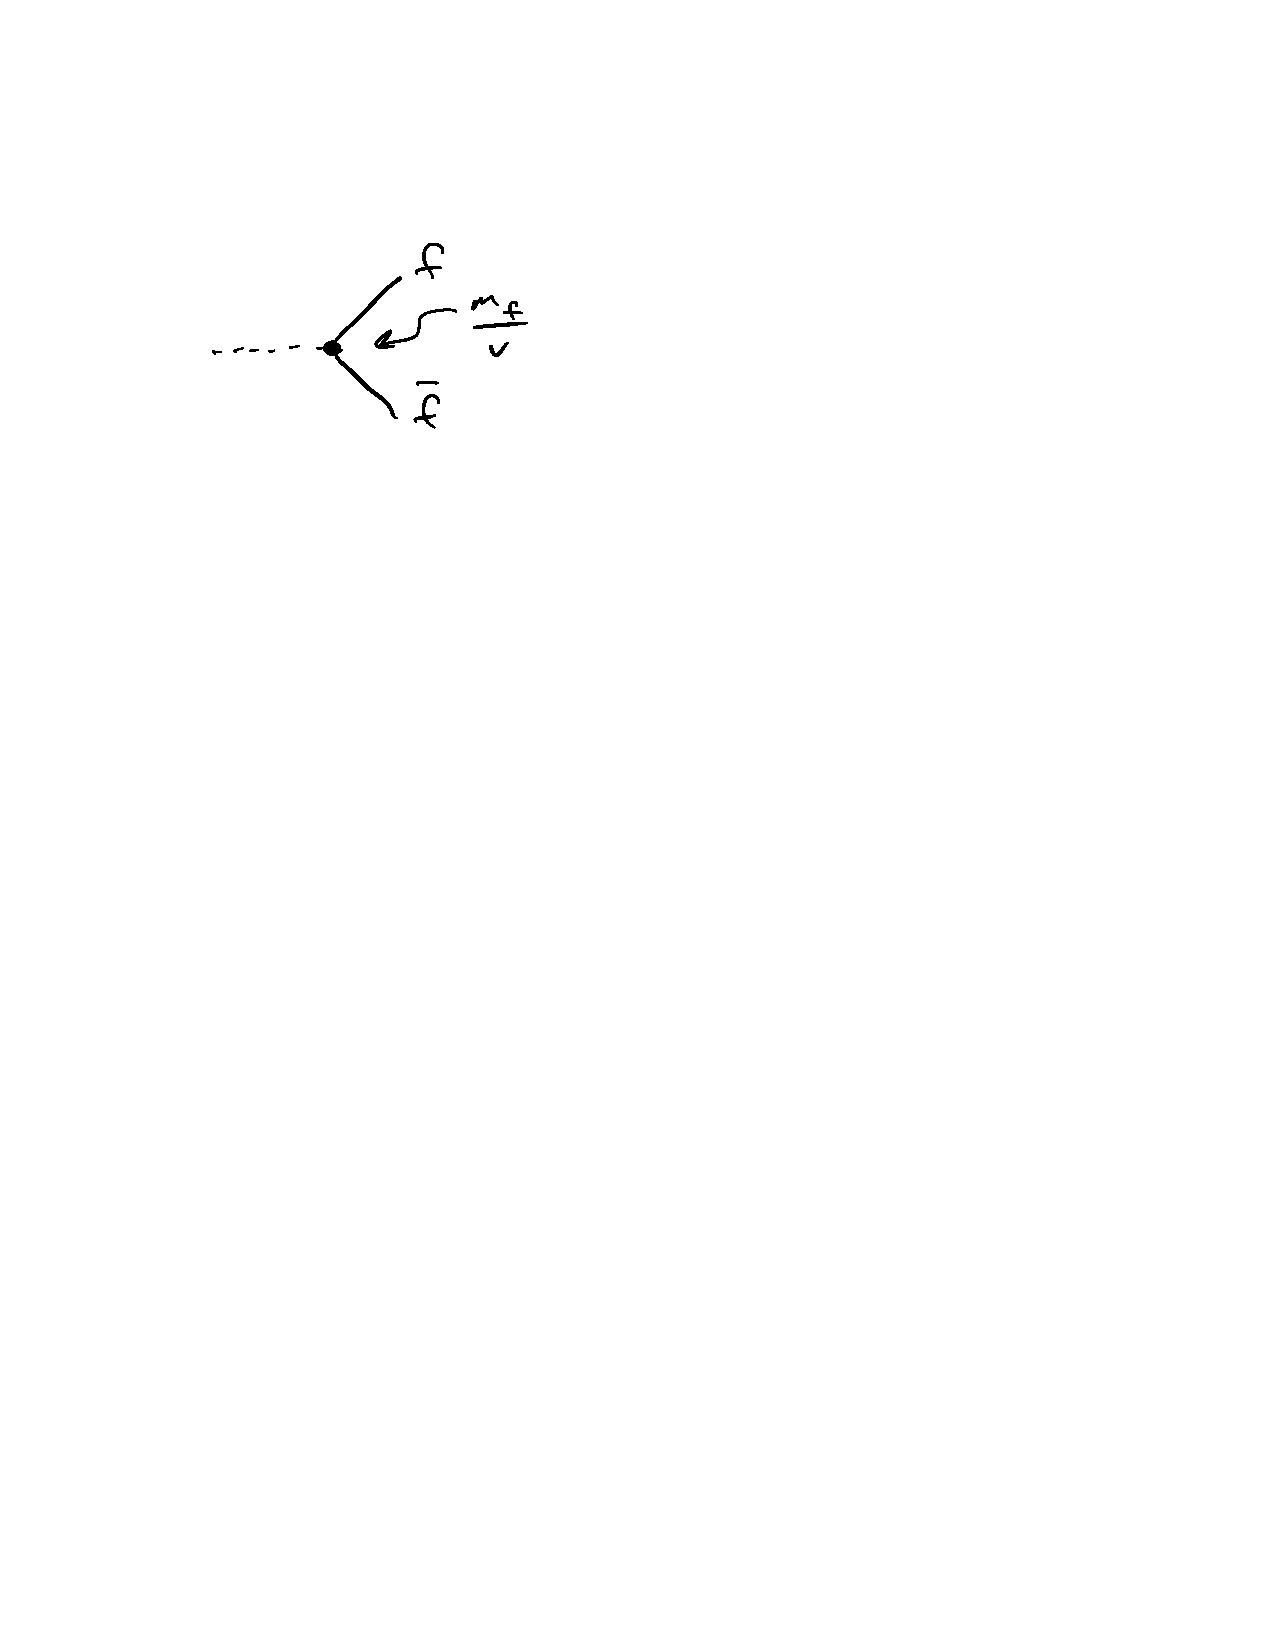
\includegraphics[width=0.2\textwidth]{./higgsYukawa.pdf}}
\ee

Can construct all massive fermions this way.

\be
g_F = \sqrt{2}\frac{m_f}{v} \hspace*{1in} v = 250 \GeV
\ee

Interestingly for the top quark:  $m_t = 173.5$  $\sqrt{2}m_t \sim v $  $g_t \sim 1 (0.997)$

Other numbers small:
\be
g_b \sim 0.03 \hspace*{1in}  g_e \sim 10^{-6}  \hspace*{1in}  g_\nu \sim 10^{-12} 
\ee

\fbox{\begin{minipage}{0.4\textwidth}
\underline{Bonus:}
\be
 \phi_c \equiv i\sigma_2 \phi^2 \rightarrow \frac{1}{\sqrt{2}} \begin{pmatrix} v+h \\ 0 \end{pmatrix}
\ee
\end{minipage}}

\lineacross

Now, how do we know any of this is correct ?
\bi
\item[-] Predicted neutral currents.  Then found.
\item[-] Predicted value of $m_W$ and $m_Z$.  Later discovered where predicted.
\ei

Other precise predictions of the electro-weak model was confronted with equally precise measurements of $W^\pm$, $Z$ properties at LEP (Large Electron Positron Collider) and Tevatron. 

Will say a few things about these tests...

\clearpage

LET produced large quantities of $e^+e^-$ collisions. 

Many ``on the Z resonance''

Any process with $\gamma$ can be replaced with Z
eg:

\be
\underbrace{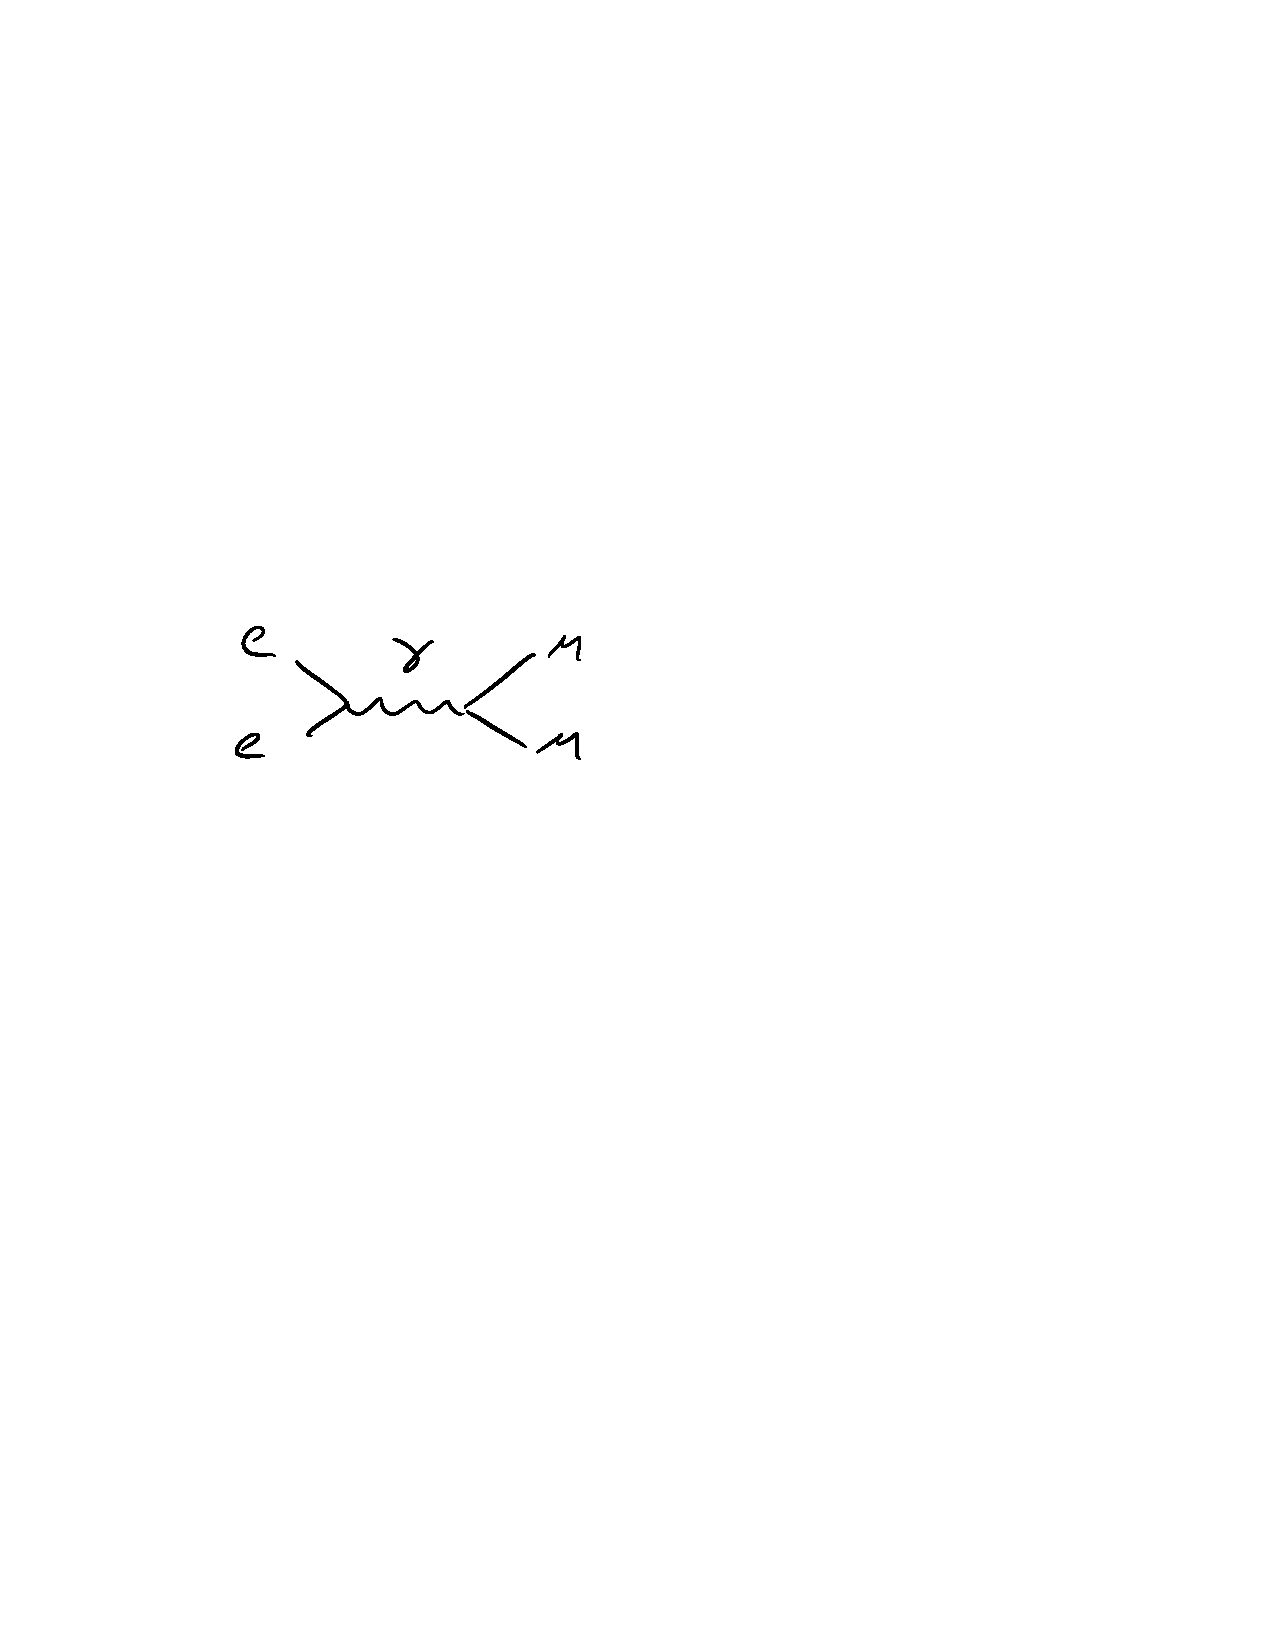
\includegraphics[width=0.4\textwidth]{./eeGammaMM.pdf}}_{\rmt{\huge $M_\gamma \sim \frac{e^2}{q^2}$ }}
\hspace*{0.5in}
\underbrace{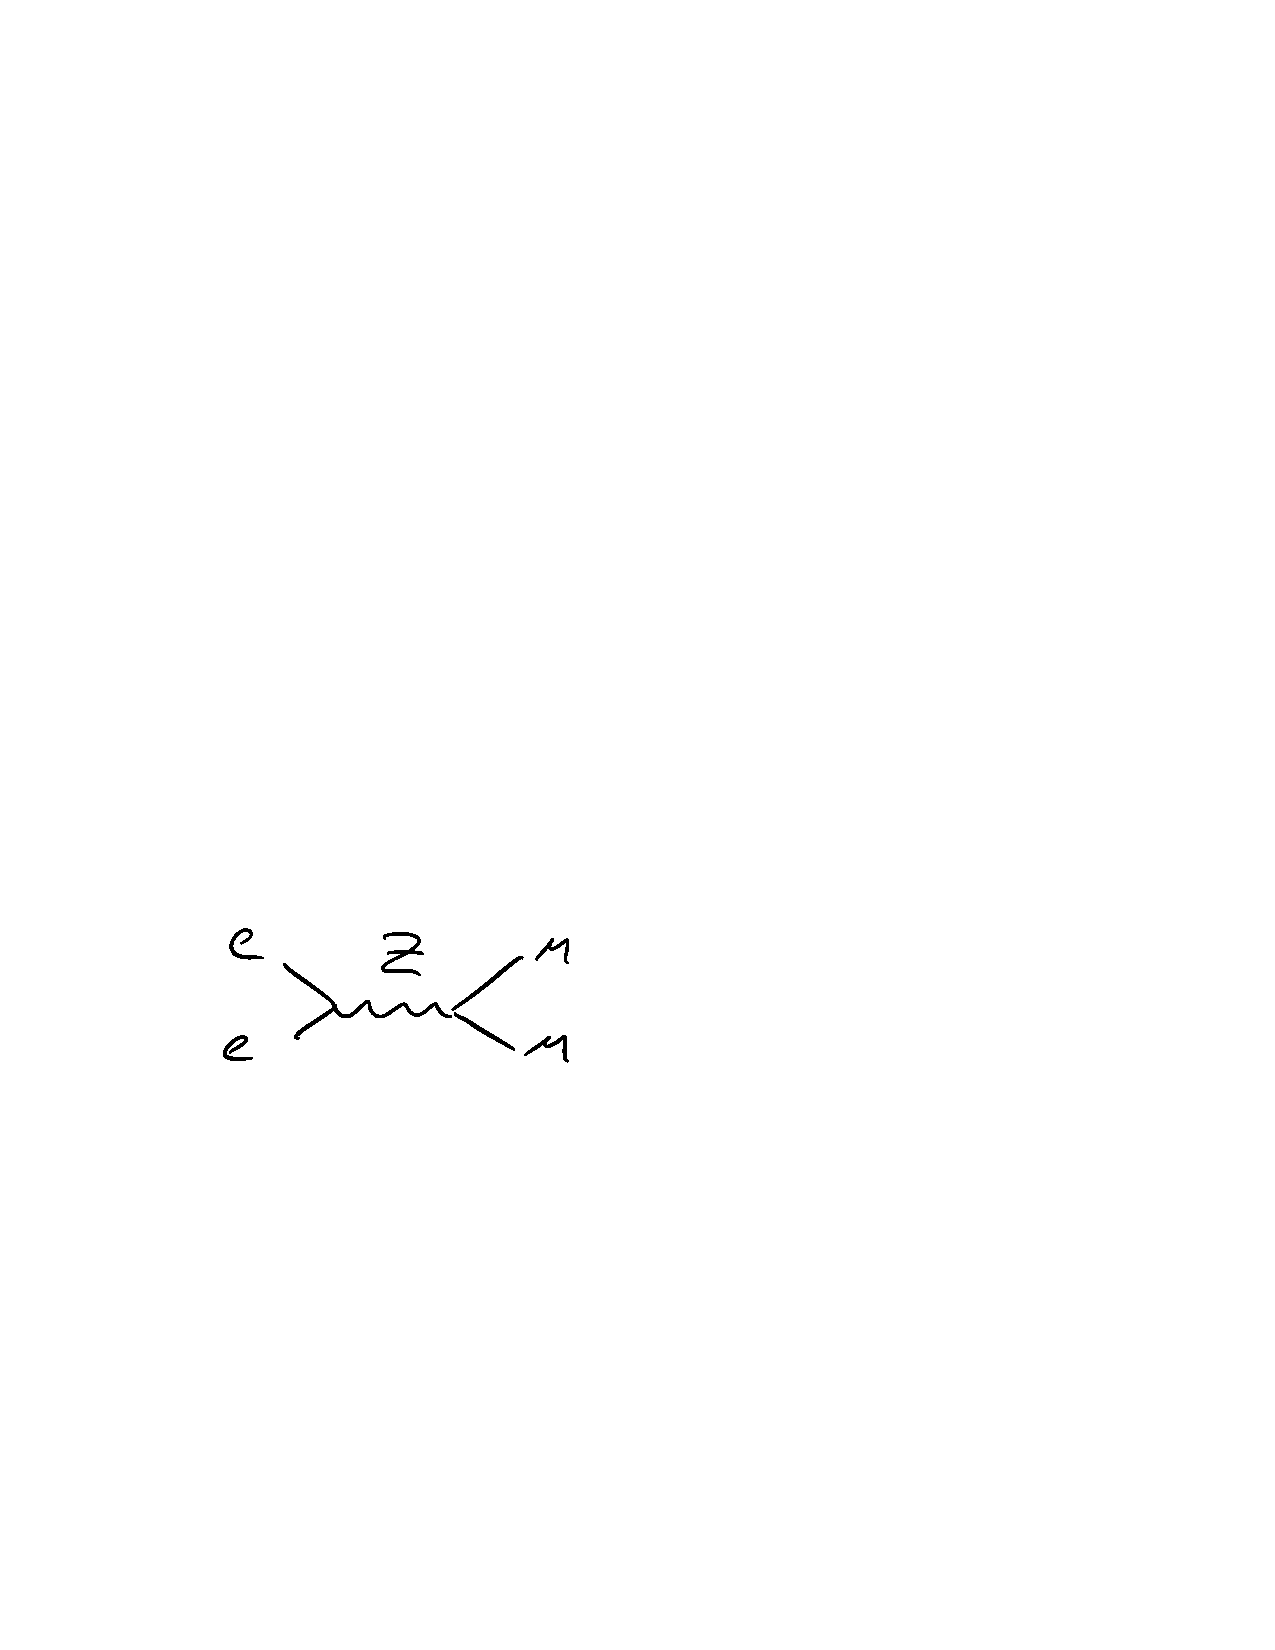
\includegraphics[width=0.4\textwidth]{./eeZMM.pdf}}_{\rmt{\huge $M_Z \sim \frac{g_Z^2}{q^2 - M_Z^2}$ }}
\ee

In these ``s-channel'' diagrams the 4-momentum of the internal line is equal to $E_{CM}$.

B/c $m_Z^2 = (90\ \GeV)^2$
\bi
\item[-] For $E_{CM}^2 << m_Z^2$:  $M_\gamma >> M_Z$  (EM dominates)
\item[-] For $E_{CM}^2 >> m_Z^2$:  $M_\gamma >> M_Z$  (Both are important $\alpha \sim \alpha_W$)
\item[-] For $E_{CM}^2 \sim m_Z^2$:  $M_Z >> M_\gamma$  (Weak Interaction (Z-boson production) dominates)
\ei

In fact, when $E_{CM} = m_Z$ is naively infinite ...  B/c doesn't account for Z being an unstable particles. 

Number of way to account for this. 

Think of the Z-boson wave-function $\psi \sim e^{imt}$ (in the Z rest frame $E\sim m$).

For unstable particle $\psi \rightarrow \psi \sim e^{imt} e^{-\Gamma t/2}$ (to account for the decay rate)

Implies $\psi^*\psi \sim e^{-\Gamma t} = e^{-\frac{t}{\tau}} $

$\Rightarrow$ unstable particles can describe by $m \rightarrow m- i\Gamma/2$

\be
m_Z^2 \rightarrow \left(m_Z^2 - \frac{i \Gamma_Z}{2}\right)^2 = m_Z^2 - im_Z \Gamma_Z - \frac{1}{4} \Gamma_Z^2
\ee

For well-defined particles $\Gamma_Z << m_Z$ $\Rightarrow $ drop terms $\mathcal{O}(\Gamma_Z)$.

So,
\be
M_Z \sim \frac{g_Z^2 }{q^2 - m_Z^2 +i m_Z \Gamma_Z}
\ee

\be
\sigma \sim |M_Z|^2 \sim \left| \frac{1 }{E_{EM}^2 - m_Z^2 +i m_Z \Gamma_Z} \right|^2 = \frac{1 }{\left(E_{EM}^2 - m_Z^2\right)^2  + m_Z^2 \Gamma_Z^2}
\ee

$\Rightarrow ee\rightarrow Z$ cross section sharply peaked at $E_{CM} = m_Z$.

This dependence on mass referred to as ``Breit-Wigner`` distribution.\\

\begin{minipage}{\textwidth}
\underline{\textbf{Cartoon of the behaviour:}}\\
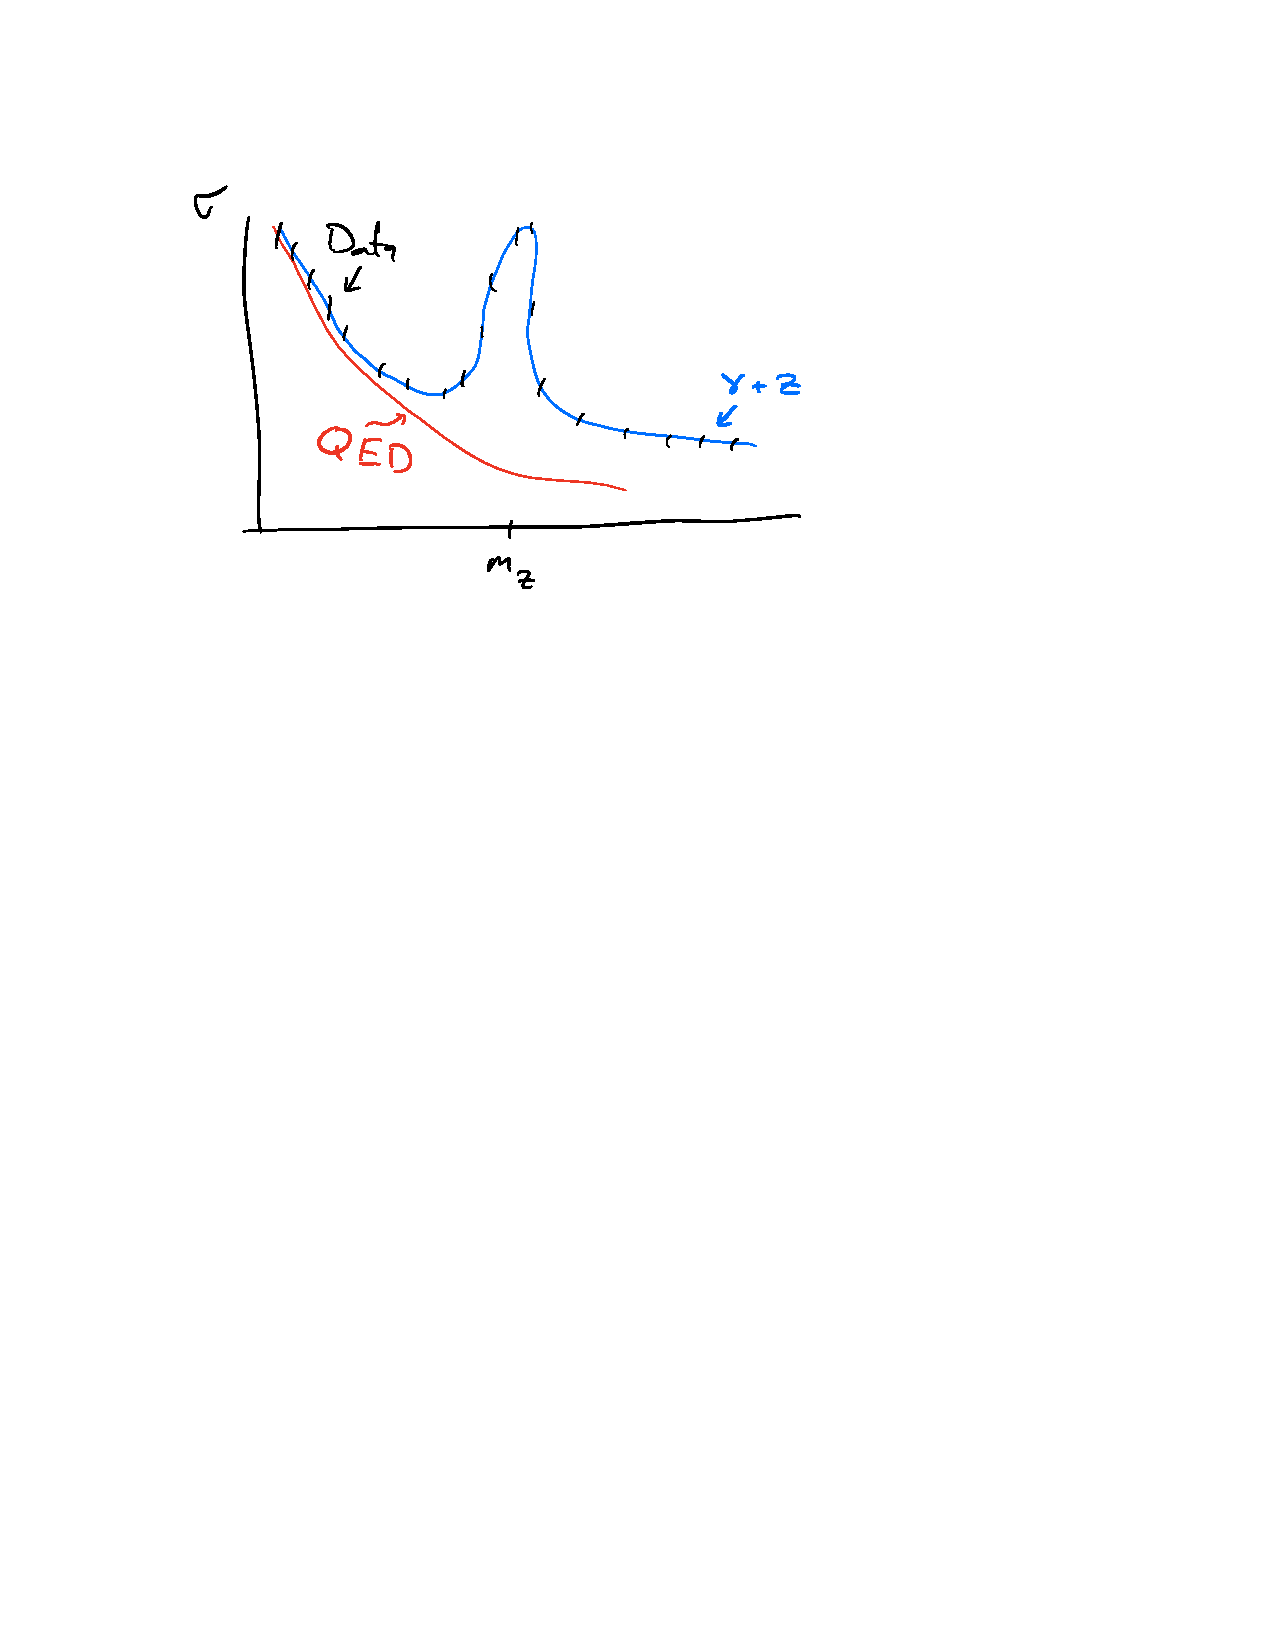
\includegraphics[width=0.99\textwidth]{./ZPeak.pdf}
\end{minipage}

\begin{minipage}{\textwidth}
\underline{\textbf{Actual data compared with Electro-weak theory:}}\\
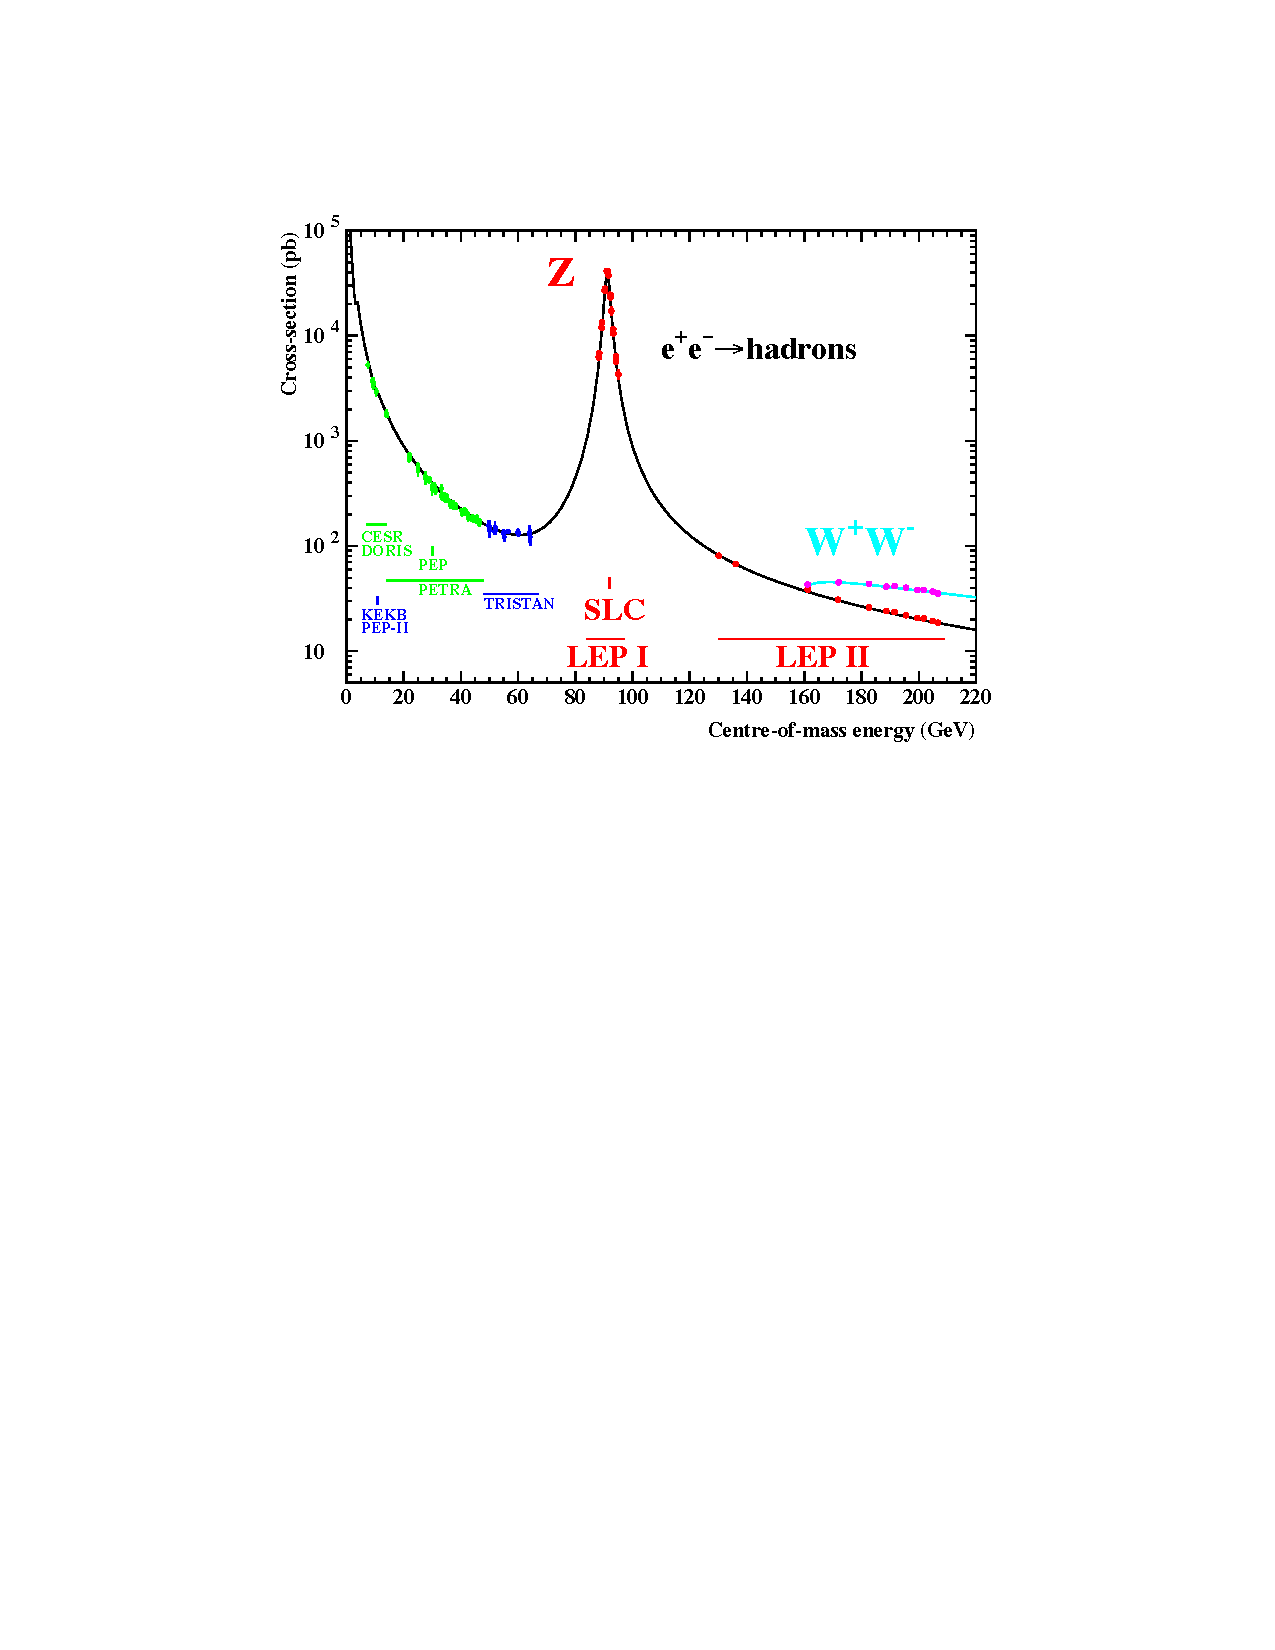
\includegraphics[width=0.99\textwidth]{./LEPData.pdf}
\end{minipage}


$m_Z$ was measured to 0.002\% precision 
\bi
\item[-] Required correcting for distortions of the earth due to the Moon
\item[-] Required correcting for electrical currents induced by French train system
\ei

Total width measured to be 
\be
\Gamma_Z = 2.4952 \pm 0.0023 \GeV
\ee

We can do something cool with this...

\underline{\textbf{Remember}}

\be
\Gamma_Z = 3 \Gamma_{\ell^+\ell^-} + \Gamma_{\rmt{hadrons}} + N_\nu \Gamma_{\nu\bar{\nu}}
\ee

Only generations observed.  
Know they come in doublets. 

Maybe there is a 4th generation which has been too heavy to be seen... $\begin{pmatrix}\nu_X \\ X \end{pmatrix}$\\
Would lead to $Z\rightarrow \nu_X\bar{\nu_X}$.


Could turn the above around to get an equation for the number of neutrinos

\be
N_\nu = \frac{\Gamma_Z - 3 \Gamma_{\ell^+\ell^-} - \Gamma_{\rmt{hadrons}}}{\Gamma_{\nu\bar{\nu}}}
\ee

\bi
\item[-] Measure $\Gamma_{\ell^+\ell^-}$ from $ee\rightarrow Z \rightarrow \mu\mu$
\item[-] Measure $\Gamma_{\rmt{hadrons}}$ from $ee\rightarrow Z \rightarrow $ jets
 \ei

\bc
\rmt{\huge $\Rightarrow N_\nu = 2.9840 \pm 0.0082 $}
\ec

Exactly 3 generation of light neutrinos ($m_\nu < m_Z/2$)! 

$\Rightarrow$ Probably only 3 generations!

}
\end{document}


